\section{Mottagningskonvertern}
\index{mottagningskonverter}
\index{konverter}
\index{mottagare!konverter}

\begin{figure}
  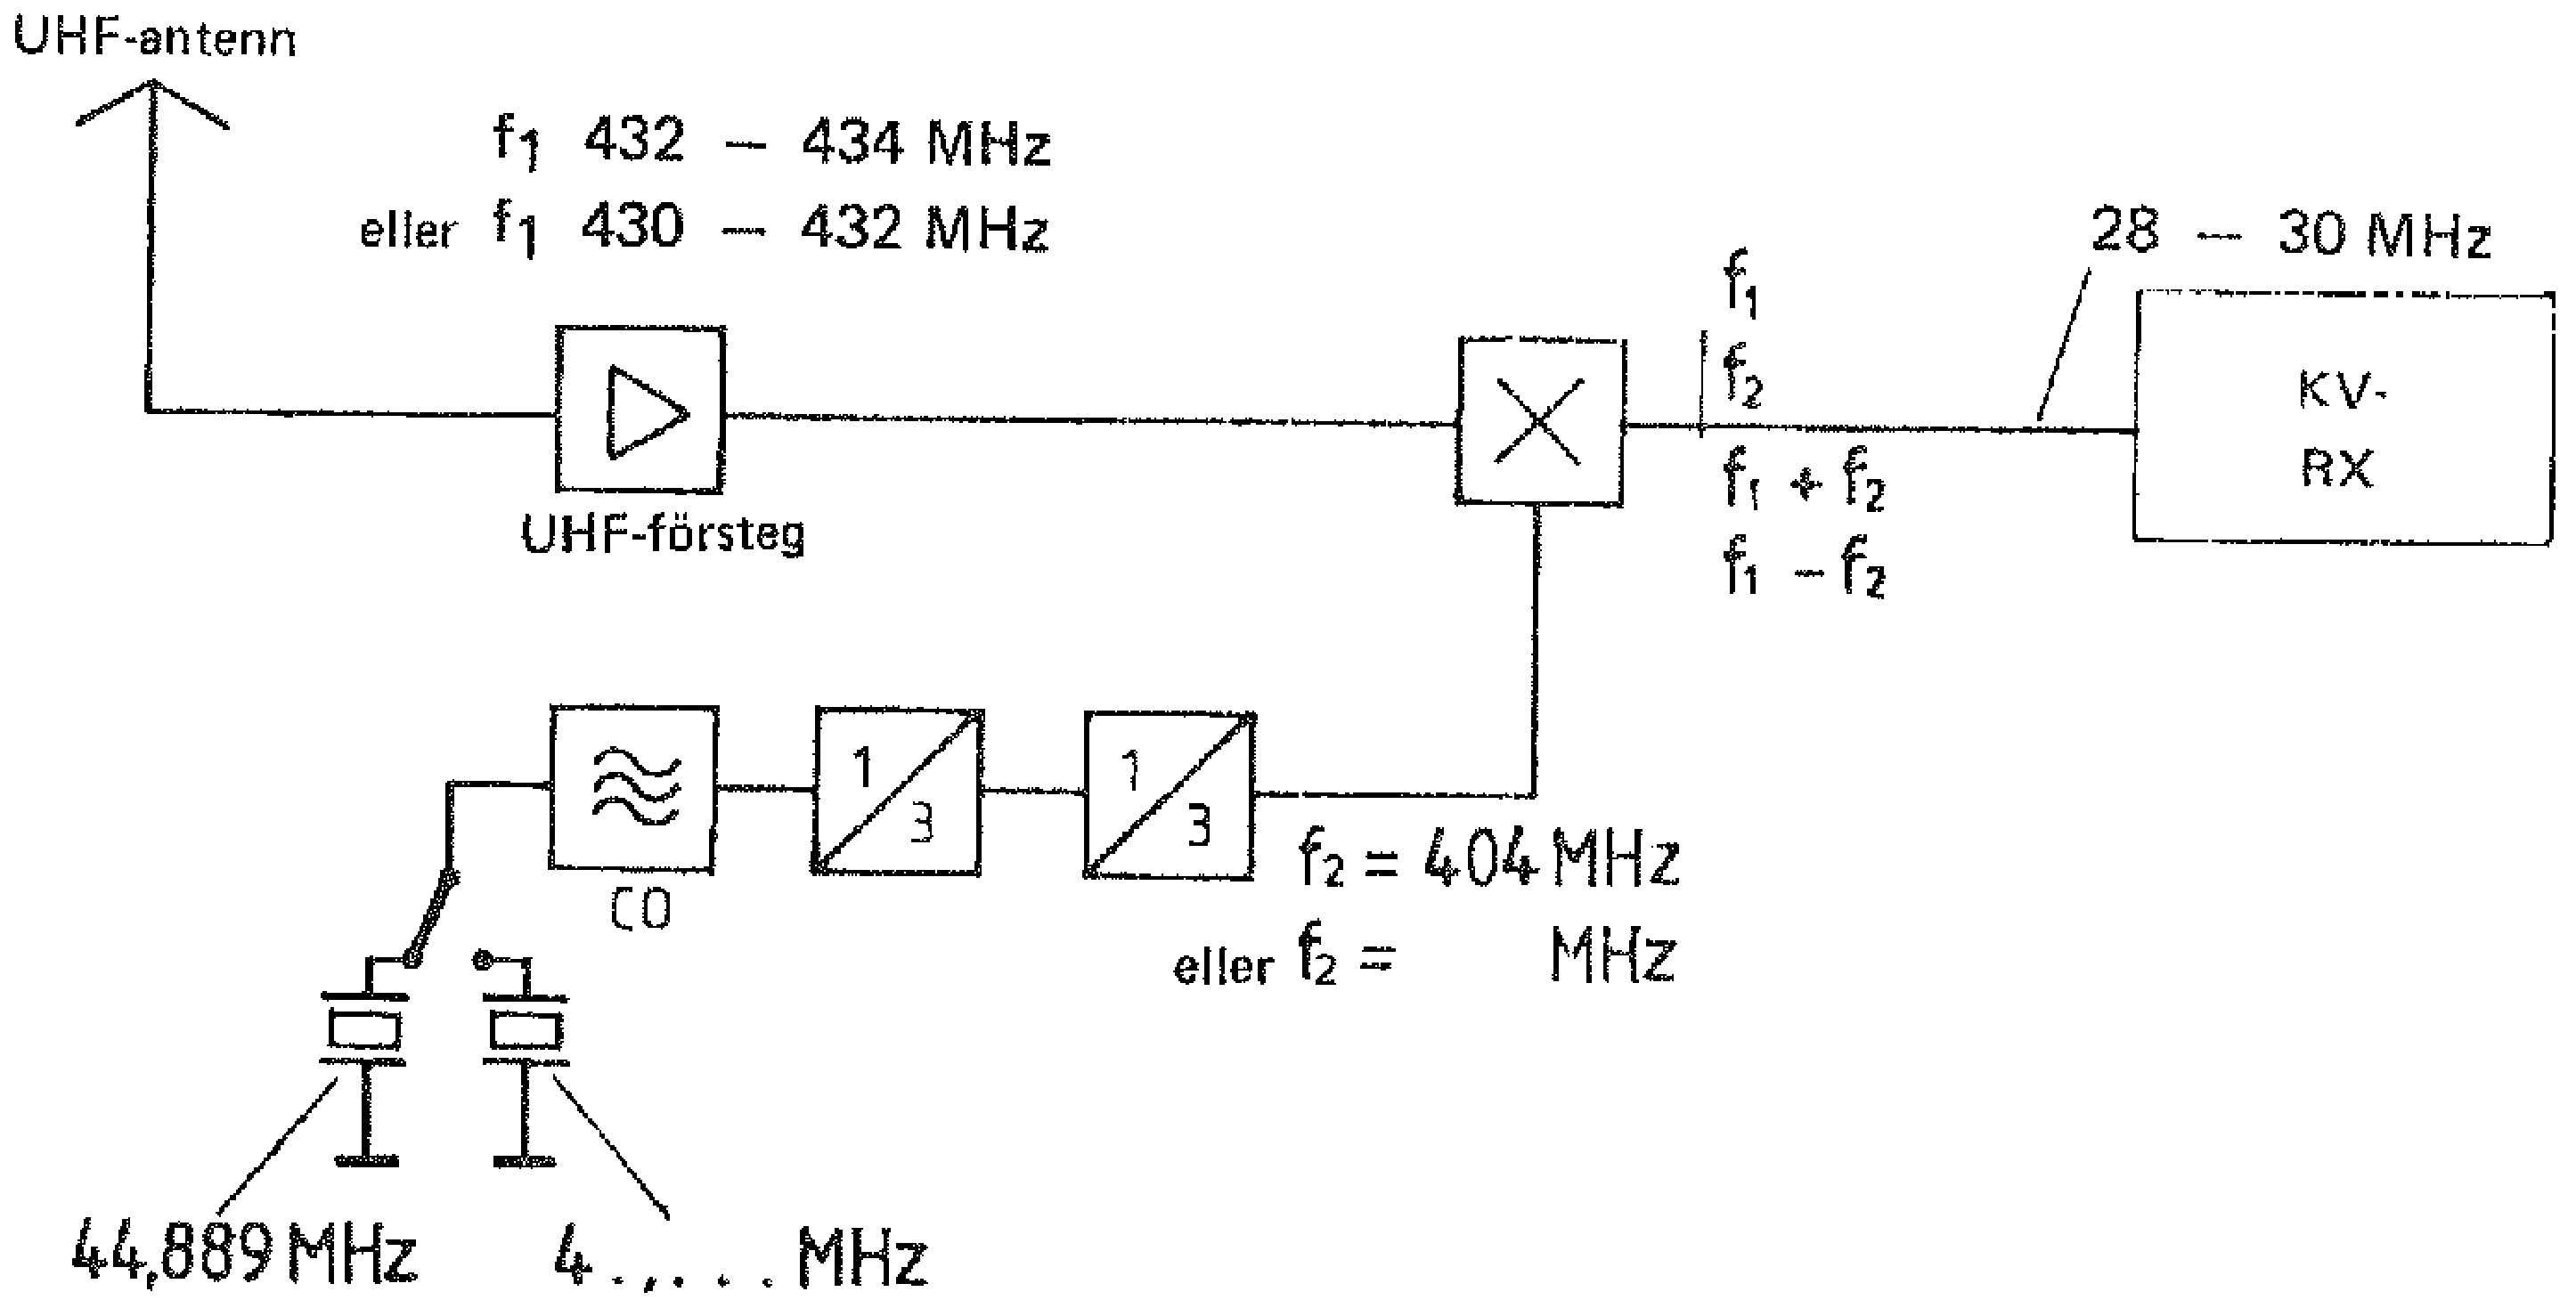
\includegraphics[width=\textwidth]{images/cropped_pdfs/bild_2_4-18.pdf}
  \caption{Mottagningskonverter UHF till KV}
  \label{fig:bildII4-18}
\end{figure}

Konverter betyder i detta sammanhang frekvensomvandlare.
När det är önskvärt att flytta över alla signalerna inom ett helt frekvensområde
till ett annat, så används en mottagningskonverter där frekvensblandning och
frekvensfilter används, så som illustreras i bild \ref{fig:bildII4-18}.

Konvertern fungerar som tillsats före en mottagare för att denna även
ska kunna användas inom ett annat frekvensområde.
I en konverter är oscillatorfrekvensen fast, medan avsökningen av
frekvensområdet görs med VFO i mottagaren.
Mellanfrekvensfiltret i mottagaren är så brett som hela det frekvensområde
som tas emot av konvertern och avsöks med mottagaren.

\textbf{Exempel:}
I en KV-mottagare för området 28--30~MHz vill man även kunna lyssna i området
432--434~MHz (UHF).
Den i konvertern mottagna UHF-signalen förstärks för att sedan blandas med
404~MHz, en frekvens som multiplicerats upp från en kristalloscillator (CO) i
konvertern.
De blandningsprodukter som filtreras fram kommer att ligga inom området
28--30~MHz och kan alltså avlyssnas i KV-mottagaren.
Övriga blandningsprodukter blir undertryckta i KV-mottagarens ingångskretsar.

Blandningsfrekvensen 404~MHz i konvertern är beräknad på följande sätt:

Mittfrekvensen i UHF-bandet är

\[\frac{432+434}{2} = 433\text{ MHz } = f_1\]

Mittfrekvensen i KV-mottagarens frekvensband är

\[\frac{28 + 30}{2} = 29\text{ MHz}\]

Med vilken frekvens \(f_2\) måste 433~MHz blandas för att erhålla en
blandningsprodukt av 29~MHz?
29~MHz är mindre än \(f_1\) , alltså kan endast skillnadsfrekvensen komma i
fråga (vid summafrekvens skulle blandningsfrekvensen bli högre än 433~MHz).

Vid användning av skillnadsfrekvensen ges två möjligheter:

\begin{gather*}
  \text{för }f_2 - f_1 = f_2 - 433 = 29\text{ MHz är }f_2 = 462\text{ MHz} \\
  \text{för }f_1 - f_ = 433 - f_2 = 29\text{ MHz är }f_2 = 404{\text MHz} \\
\end{gather*}

Vi bestämmer oss för alternativet 404~MHz av ett speciellt skäl.
Här motsvaras den högsta UHF-frekvensen 434~MHz av \(434 - 404 = 30\)~MHz
och den lägsta UHF-frekvensen 432~MHz av \(432 - 404 = 28\)~MHz.
På så sätt kan kHz-graderingen på KV-mottagarens skala användas direkt utan
omräkning.

Fördelen med en konverter är att kostnaden för en sådan är låg jämfört
med den för en komplett mottagare för ett tillkommande band.
Förutsättningen är att en mottagare redan finns.

Nackdelen är att mottagaren inte samtidigt kan användas för sin
ordinarie funktion.
